\documentclass{article}
\usepackage[utf8]{inputenc}
\usepackage{geometry}
\usepackage{multirow}
 \geometry{
 a4paper,
 total={170mm,257mm},
 left=20mm,
 top=20mm,
 }
 \usepackage{graphicx}
 \usepackage{titling}

 \title{Internet of Things: Interconnections and Intelligence}
\author{Malathi M}
\date{January 2023}
 
 \usepackage{fancyhdr}
\fancypagestyle{plain}{%  the preset of fancyhdr 
    \fancyhf{} % clear all header and footer fields
    \fancyfoot[R]{
\includegraphics[width=2cm]{Untitled-1.png}}
    \fancyfoot[L]{\thedate}
    \fancyhead[L]{IoT Architectures, Protocols, and Applications}
    \fancyhead[R]{\theauthor}
}
\makeatletter
\def\@maketitle{%
  \newpage
  \null
  \vskip 1em%
  \begin{center}%
  \let \footnote \thanks
    {\LARGE \@title \par}%
    \vskip 1em%
    %{\large \@date}%
  \end{center}%
  \par
  \vskip 1em}
\makeatother

\usepackage{lipsum}  
\usepackage{cmbright}

\begin{document}

\maketitle

\noindent\begin{tabular}{@{}ll}
    Student: \theauthor\\
    Registration No: 21011101072\\
    Class: AI\&DS - A\\
\end{tabular}

\section*{IoT - Internet of Things}
One of the popular definition of Internet of Things is that, it is simply an interaction between the physical and digital worlds, i.e., the digital world interacts with the physical world using a plethora of sensors and actuators. Another definition defines the Internet if Things as a paradigm in which computing and networking capabilities are embedded in any kind of conceivable object.\\
Hence IoT is a world of devices and appliances which are equipped with sensors, actuators, processors, and transceivers, that acquire data at large amounts which can be used collaboratively to achieve complex tasks that require a high degree of intelligence.\\
The storage, processing capabilities and communication of an IoT object are pretty much restricted and constrained owing to the resources available at the moment. Hence the main research challenge is to ensure that we get the right kind of data at the desired level of accuracy. 


\section*{Architecture Of IoT}
\vspace{1em}
        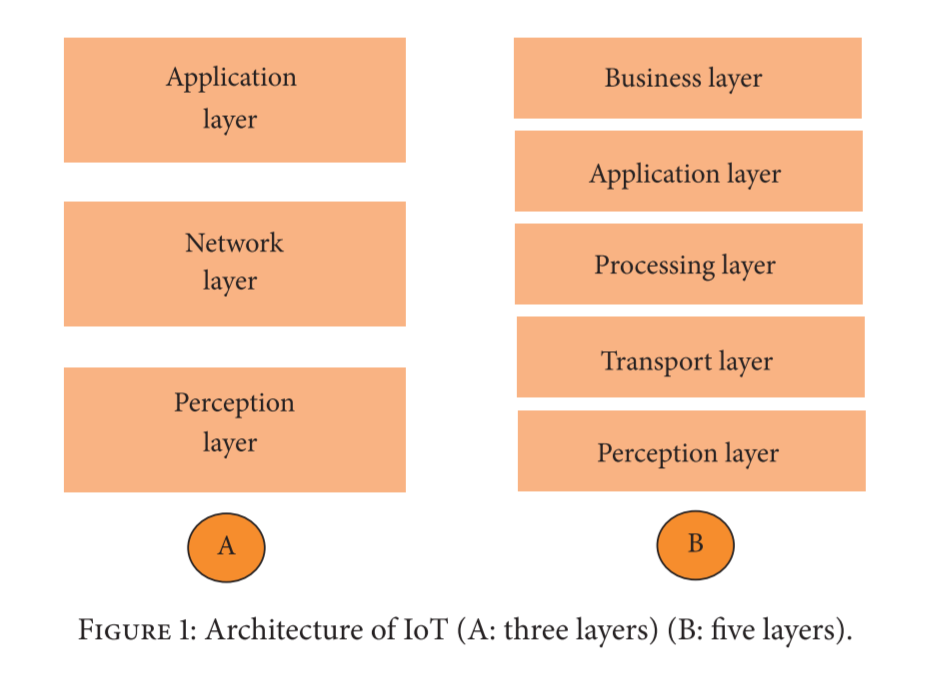
\includegraphics[width=0.7\linewidth]{fig1.png}
\vspace{1em}\\
There is no single defined architecture for IoT, the most basic architecture is the three layer architecture and the five layer architecture just includes transport layer and business layer.\\

1. PERCEPTION LAYER\\
It is the physical layer that consists of sensors for sensing and collecting information about the environment\\

2. NETWORK LAYER\\
It is responsible for the interconnection between the smart objects and the servers. It is also used for transmitting and processing data collected by the sensors\\

3. TRANSPORT LAYER\\
This layer transfers the sensor data from the perception layer to the processing layer and vice versa through networks such as wireless, 3G, LAN, Bluetooth, RFID, and NFC.\\

4. PROCESSING LAYER\\
Also known as the middleware layer. It stores, analyzes , and processes huge amount of data that comes from the transport layer.\\

5. APPLICATION LAYER\\
It defines various applications in which the IoT can be deployed. for example, smart homes, smart cities, and smart health\\

6. BUSINESS LAYER \\
It manages the whole IoT system, including applications, business and profit models, and users’ privacy.\\


\section*{Sensors and Actuators}
All IoT objects need to have one or more sensors, so that they can interact with the physical environment and collect data, hence having context awareness. Context awareness cannot be achieved without sensor technology. IoT sensors are mostly small in size, low cost and consume less power, hence they are constrained by other factors like battery capacity and ease of deployment. Commonly used sensors include Mobile phone based sensors, Medical sensors, Neural sensors, Environmental and Chemical sensors and Radio Frequency Identification (RFID).\\
Actuators are devices that are capable of effecting a change in the environment by converting electrical energy into some form of useful energy like heating or cooling elements, speakers, lights, displays and motors.


\section*{Preprocessing}
As the smart things collect huge amount of data every moment, these data require cloud based resources because the cloud offers massive data handling, scalability and flexibility. But since this is not sufficient for many present IoT devices.\\
Hence a Smart Gateway is present between the cloud and the smart things. This smart gateway collects data, preprocess and filters the collected data, storage and networking services to IoT devices, communicating with the cloud and sending only necessary data, monitoring power consumption of IoT devices, monitoring activities and services of IoT devices, and ensuring security and privacy of data.


\section*{Communication}
The Internet of Things is a large number of heterogeneous smart devices connecting to the internet. To achieve a complex task we need the devices to work together collaboratively, hence they need to communicate. IoT devices typically connect to the Internet through the IP (Internet Protocol) stack. This stack is very complex and demands a large amount of power and memory from the connecting devices. The IoT devices can also connect locally through non-IP networks, which consume less power, and connect to the Internet via a smart gateway.

\section*{Middleware}
Ubiquitous computing is the main idea of IoT, that is incorporating computing and connectivity in all the things around us.Interoperability of such heterogeneous devices needs well-defined standards. But standardization is difficult because of the varied requirements of different applications and devices. For such heterogeneous applications, the solution is to have a middleware platform, which will abstract the details of the things for applications. That is, it will hide the details of the smart things. Middleware acts as a software bridge hence providing an Application Programming Interface (API) for communications, data management, computation, security and privacy.
\\
\\
\section*{Applications of IoT}
\vspace{1em}
        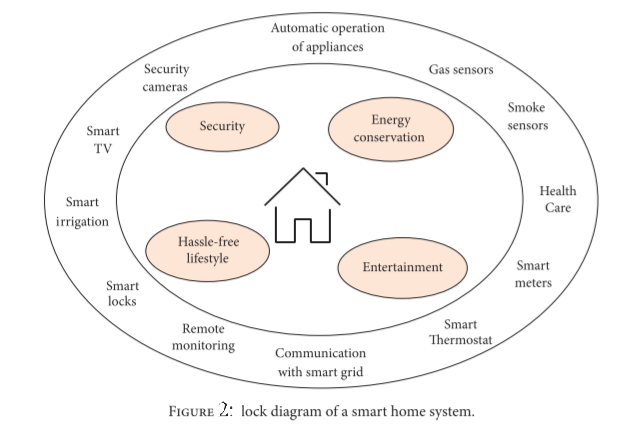
\includegraphics[width=0.8\linewidth]{fig2.png}
\vspace{1em}\\
There are a lot of intelligent applications developed that can be used in diverse areas in our day to day life, but all of them are not readily available. However, the application smart homes is becoming more popular due to the sensor and actuators technologies which have significantly improved.\\
Other places of IoT applications:\\
1. Smart Cities\\
2. Social Life and Entertainment\\
3. Health and Fitness\\
4. Smart Environment and Agriculture\\
5. Supply Chain and Logistics\\
6. Energy Conservation\\
\\

\begin{tabular}{|p{3cm}|p{10cm}|}
\hline
ASPECT & CHALLENGES \\ \hline
Sensors & Even though GPS, sleep trackers, heartbeat monitors etc help us in our day to day lives, and is being used to study different kinds of human behaviour to improve the quality of human life, they are also viewed as devices that invade privacy. \\ \hline
Processing & Cloud resources are not sufficient due to mobility of smart devices, real time actuation, scalability and power constraints. \\ \hline
Communication & Since IoT devices are battery powered, with minimal compute and storage resources. Due to their constrained nature communication challenges include Addressing and identification, Low power communication, Routing protocols, High speed and nonlossy communication. \\ \hline
Middleware & The challenges, which are addressed by any IoT middleware are Interoperability and programming abstractions, Device discovery and management, Big data analytics, Cloud services and scalability, and Context detection. \\ \hline
\end{tabular}


\end{document}
